\chapter{Исследования 2D}
\section{Предварительное описание}

Проведем сначала тестирование разработанной программы по векторному МКЭ на работоспособность. Образец расчетной области изображен на рисунке \ref{fig:exampleOfArea}. Это область $\Omega = [0.0, 2.0]_x \times [0.0, 2.0]_y$, она содержит 12 ребер, на всех границах будем задавать первые краевые условия. Середины наших элементов обозначены красным цветом, в этих точках мы будем рассматривать точность наших решений для оценки точности программы. 

\begin{figure}
	\centering
	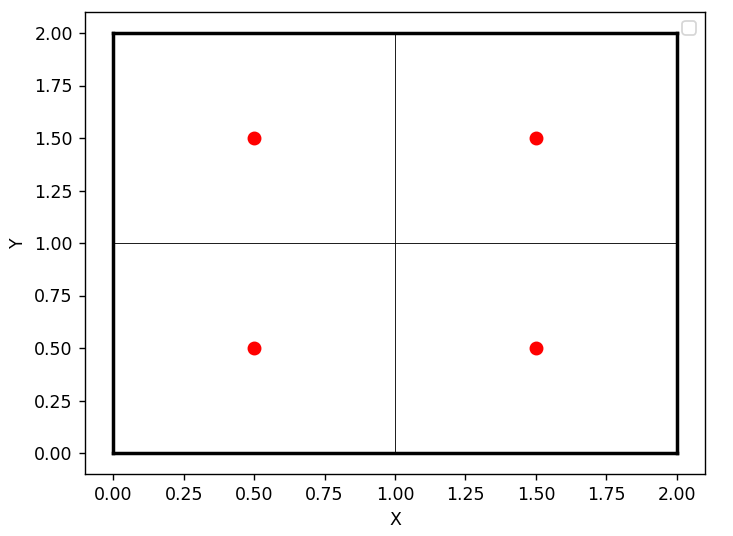
\includegraphics[width=1.0\linewidth]{images/2D_grid_example.png}
	\caption{Расчетная область}
	\label{fig:example2OfArea}
\end{figure}

\section{Тестирование на порядок аппроксимации}

Тестирование будем проводить на дифференциальном уравнении (\ref{eq_2_1}) :

\begin{equation} \label{eq_2_1}
	\text{rot} \left(\frac{1}{\mu} \text{rot} \overrightarrow{\textbf{A}}\right) + \gamma \overrightarrow{\textbf{A}} = \overrightarrow{\textbf{F}}
\end{equation}

\begin{table}
	\caption{Тестирование при $\overrightarrow{\textbf{A}} = (1.0, 1.0)^{\text{T}}$, $\overrightarrow{\textbf{F}} = (1.0, 1.0)^{\text{T}}$, $\mu = 1$, $\gamma = 1$}
	\centering
	\small
	\begin{tabularx}{1.0\textwidth}{| >{\raggedright\arraybackslash}X | >{\raggedright\arraybackslash}X | >{\raggedright\arraybackslash}X |>{\raggedright\arraybackslash}X |}
		\hline
		\centering{Точка} & \centering{Значение} & \centering{Абсолютная погрешность} & \centering{Относительная погрешность} \tabularnewline \hline		
		
		\centering{(0.5; 0.5)} & \centering{1.00000000E+000; 1.00000000E+000}& \centering{2.22044605E-016; 2.22044605E-016} & \centering{2.22044605E-016; 2.22044605E-016} \tabularnewline \hline
		
		\centering{(1.5; 0.5)} & \centering{1.00000000E+000; 1.00000000E+000}& \centering{2.22044605E-016; 2.22044605E-016} & \centering{2.22044605E-016; 2.22044605E-016} \tabularnewline \hline
		
		\centering{(0.5; 1.5)} & \centering{1.00000000E+000; 1.00000000E+000}& \centering{2.22044605E-016; 2.22044605E-016} & \centering{2.22044605E-016; 2.22044605E-016} \tabularnewline \hline
		
		\centering{(1.5; 1.5)} & \centering{1.00000000E+000; 1.00000000E+000}& \centering{2.22044605E-016; 2.22044605E-016} & \centering{2.22044605E-016; 2.22044605E-016} \tabularnewline \hline
		
	\end{tabularx}
	\label{tab:test9}
\end{table}

\begin{table}
	\caption{Тестирование при $\overrightarrow{\textbf{A}} = (y, x)^{\text{T}}$, $\overrightarrow{\textbf{F}} = (y, x)^{\text{T}}$, $\mu = 1$, $\gamma = 1$}
	\centering
	\small
	\begin{tabularx}{1.0\textwidth}{| >{\raggedright\arraybackslash}X | >{\raggedright\arraybackslash}X | >{\raggedright\arraybackslash}X |>{\raggedright\arraybackslash}X |}
		\hline
		\centering{Точка} & \centering{Значение} & \centering{Абсолютная погрешность} & \centering{Относительная погрешность} \tabularnewline \hline		
		
		\centering{(0.5; 0.5)} & \centering{5.00000000E-001; 5.00000000E-001}& \centering{0.00000000E+000; 0.00000000E+000} & \centering{0.00000000E+000; 0.00000000E+000} \tabularnewline \hline
		
		\centering{(1.5; 0.5)} & \centering{1.50000000E+000; 5.00000000E-001}& \centering{0.00000000E+000; 0.00000000E+000} & \centering{0.00000000E+000; 0.00000000E+000} \tabularnewline \hline
		
		\centering{(0.5; 1.5)} & \centering{5.00000000E-001; 1.50000000E+000}& \centering{0.00000000E+000; 0.00000000E+000} & \centering{0.00000000E+000; 0.00000000E+000} \tabularnewline \hline
		
		\centering{(1.5; 1.5)} & \centering{1.50000000E+000; 1.50000000E+000}& \centering{0.00000000E+000; 0.00000000E+000} & \centering{0.00000000E+000; 0.00000000E+000} \tabularnewline \hline
		
	\end{tabularx}
	\label{tab:test10}
\end{table}

\begin{table}
	\caption{Тестирование при $\overrightarrow{\textbf{A}} = (1 + y + x; 1 + x)^{\text{T}}$, $\overrightarrow{\textbf{F}} = (1 + y + x; 1 + x)^{\text{T}}$, $\mu = 1$, $\gamma = 1$}
	\centering
	\small
	\begin{tabularx}{1.0\textwidth}{| >{\raggedright\arraybackslash}X | >{\raggedright\arraybackslash}X | >{\raggedright\arraybackslash}X |>{\raggedright\arraybackslash}X |}
		\hline
		\centering{Точка} & \centering{Значение} & \centering{Абсолютная погрешность} & \centering{Относительная погрешность} \tabularnewline \hline		
		
		\centering{(0.5; 0.5)} & \centering{2.00000000E+000; 1.50000000E+000}& \centering{4.44089210E-016; 0.00000000E+000} & \centering{2.22044605E-016; 0.00000000E+000} \tabularnewline \hline
		
		\centering{(1.5; 0.5)} & \centering{3.00000000E+000; 2.50000000E+000}& \centering{4.44089210E-016; 4.44089210E-016} & \centering{1.48029737E-016; 1.77635684E-016} \tabularnewline \hline
		
		\centering{(0.5; 1.5)} & \centering{3.00000000E+000; 1.50000000E+000}& \centering{8.88178420E-016; 0.00000000E+000} & \centering{2.96059473E-016; 0.00000000E+000} \tabularnewline \hline
		
		\centering{(1.5; 1.5)} & \centering{4.00000000E+000; 2.50000000E+000}& \centering{8.88178420E-016; 4.44089210E-016} & \centering{2.22044605E-016; 1.77635684E-016} \tabularnewline \hline
		
	\end{tabularx}
	\label{tab:test11}
\end{table}

\begin{table}
	\caption{Тестирование при $\overrightarrow{\textbf{A}} = (y^2; x^2)^{\text{T}}$, $\overrightarrow{\textbf{F}} = (y^2 - 2; x^2 - 2)^{\text{T}}$, $\mu = 1$, $\gamma = 1$}
	\centering
	\small
	\begin{tabularx}{1.0\textwidth}{| >{\raggedright\arraybackslash}X | >{\raggedright\arraybackslash}X | >{\raggedright\arraybackslash}X |>{\raggedright\arraybackslash}X |}
		\hline
		\centering{Точка} & \centering{Значение} & \centering{Абсолютная погрешность} & \centering{Относительная погрешность} \tabularnewline \hline		
		
		\centering{(0.5; 0.5)} & \centering{5.00000000E-001; 5.00000000E-001}& \centering{2.50000000E-001; 2.50000000E-001} & \centering{1.00000000E+000; 1.00000000E+000} \tabularnewline \hline
		
		\centering{(1.5; 0.5)} & \centering{5.00000000E-001; 2.50000000E+000}& \centering{2.50000000E-001; 2.50000000E-001} & \centering{1.00000000E+000; 1.11111111E-001} \tabularnewline \hline
		
		\centering{(0.5; 1.5)} & \centering{2.50000000E+000; 5.00000000E-001}& \centering{2.50000000E-001; 2.50000000E-001} & \centering{1.11111111E-001; 1.00000000E+000} \tabularnewline \hline
		
		\centering{(1.5; 1.5)} & \centering{2.50000000E+000; 2.50000000E+000}& \centering{2.50000000E-001; 2.50000000E-001} & \centering{1.11111111E-001; 1.11111111E-001} \tabularnewline \hline
		
	\end{tabularx}
	\label{tab:test12}
\end{table}

Порядок аппроксимации равен 1.


\section{Тестирование на порядок сходимости}

\begin{table}
	\caption{Тестирование при $\overrightarrow{\textbf{A}} = (\text{e}^y; \text{e}^x)^{\text{T}}$, $\overrightarrow{\textbf{F}} = (0; 0)^{\text{T}}$, $\mu = 1$, $\gamma = 1$}
	\centering
	\small
	\begin{tabularx}{1.0\textwidth}{| >{\raggedright\arraybackslash}X | >{\raggedright\arraybackslash}X | >{\raggedright\arraybackslash}X |}
		\hline
		Точка & Относительная погрешность & Порядок $\text{log}_2 \left( \frac{\Delta{i-1}}{\Delta_i} \right)$ \\ \hline
		\multirow{5}{*}{($\,^4/_3$; $\,^4/_3$)} & \centering{1.0993868E-001 1.0993868E-001} & --- \\
		\cline{2-3}	& \centering{2.0790345E-002 2.0790345E-002} & 2.403 \\
		\cline{2-3}	& \centering{5.7022633E-003 5.7022633E-003} & 1.866 \\
		\cline{2-3}	& \centering{1.3475413E-003 1.3475413E-003} & 2.081 \\
		\cline{2-3}	& \centering{3.4561228E-004 3.4561228E-004} & 1.963 \\ \hline
	\end{tabularx}
	\label{tab:test13}
\end{table}

Можем увидеть, что порядок сходимости равен 2.

\chapter{Исследования 3D}

\section{Предварительное описание}

Проведем сначала тестирование разработанной программы по векторному МКЭ на работоспособность. Образец расчетной области изображен на рисунке \ref{fig:exampleOfArea}. Это область $\Omega = [0.0, 2.0]_x \times [0.0, 2.0]_y \times [0.0, 2.0]_z$, она содержит 54 ребра, на всех границах будем задавать первые краевые условия. Середины наших элементов обозначены красным цветом, в этих точках мы будем рассматривать точность наших решений для оценки точности программы. 

\begin{figure}
	\centering
	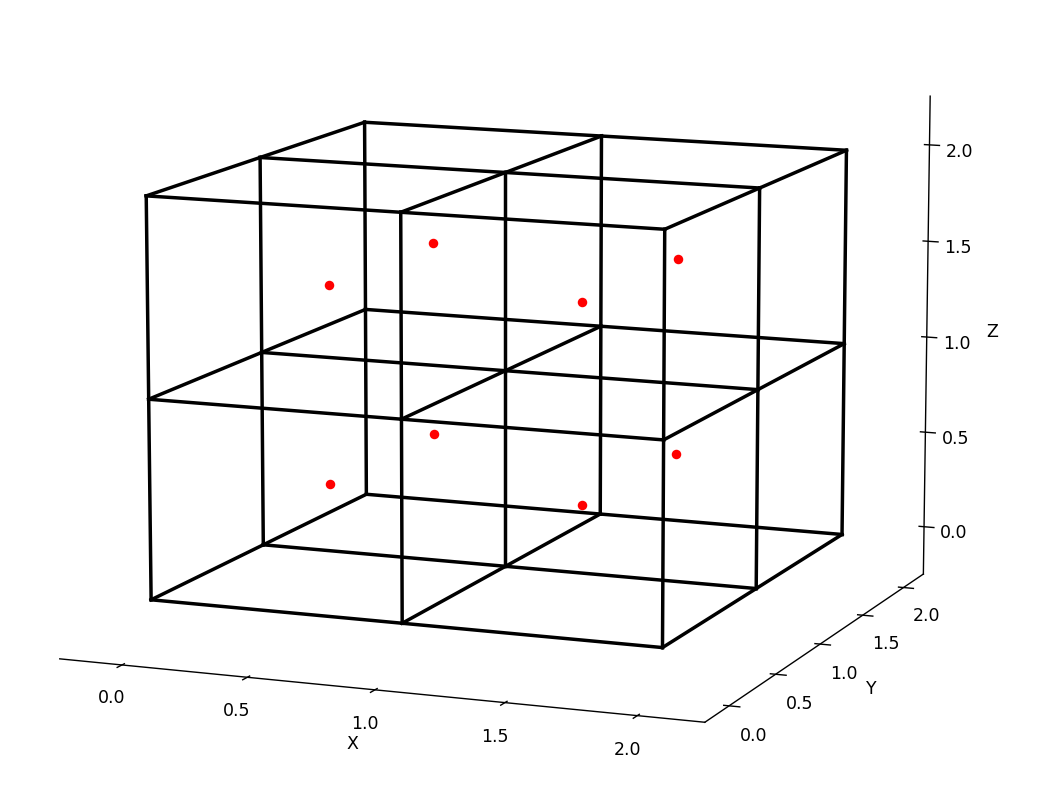
\includegraphics[width=1.0\linewidth]{images/3D_grid_example.png}
	\caption{Расчетная область}
	\label{fig:exampleOfArea}
\end{figure}

\section{Тестирование на порядок аппроксимации}

Тестирование будем проводить на дифференциальном уравнении (\ref{eq_2_1}) :

\begin{equation} \label{eq_2_1}
	\text{rot} \left(\frac{1}{\mu} \text{rot} \overrightarrow{\textbf{A}}\right) + \gamma \overrightarrow{\textbf{A}} = \overrightarrow{\textbf{F}}
\end{equation}

\begin{table}
	\caption{Тестирование при $\overrightarrow{\textbf{A}} = (1.0, 1.0, 1.0)^{\text{T}}$, $\overrightarrow{\textbf{F}} = (1.0, 1.0, 1.0)^{\text{T}}$, $\mu = 1$, $\gamma = 1$}
	\centering
	\small
	\begin{tabularx}{1.0\textwidth}{| >{\raggedright\arraybackslash}X | >{\raggedright\arraybackslash}X | >{\raggedright\arraybackslash}X |>{\raggedright\arraybackslash}X |}
		\hline
		\centering{Точка} & \centering{Значение} & \centering{Абсолютная погрешность} & \centering{Относительная погрешность} \tabularnewline \hline		

		 \centering{(0.5; 0.5; 0.5)} & \centering{1.00000000E+000; 1.00000000E+000; 1.00000000E+000}& \centering{0.00000000E+000; 0.00000000E+000; 0.00000000E+000} & \centering{0.00000000E+000; 0.00000000E+000; 0.00000000E+000} \tabularnewline \hline
	
		 \centering{(1.5; 0.5; 0.5)} & \centering{1.00000000E+000; 1.00000000E+000; 1.00000000E+000}& \centering{0.00000000E+000; 0.00000000E+000; 0.00000000E+000} & \centering{0.00000000E+000; 0.00000000E+000; 0.00000000E+000} \tabularnewline \hline

		 \centering{(0.5; 1.5; 0.5)} & \centering{1.00000000E+000; 1.00000000E+000; 1.00000000E+000}& \centering{0.00000000E+000; 0.00000000E+000; 0.00000000E+000} & \centering{0.00000000E+000; 0.00000000E+000; 0.00000000E+000} \tabularnewline \hline

		 \centering{(1.5; 1.5; 0.5)} & \centering{1.00000000E+000; 1.00000000E+000; 1.00000000E+000}& \centering{0.00000000E+000; 0.00000000E+000; 0.00000000E+000} & \centering{0.00000000E+000; 0.00000000E+000; 0.00000000E+000} \tabularnewline \hline

		 \centering{(0.5; 0.5; 1.5)} & \centering{1.00000000E+000; 1.00000000E+000; 1.00000000E+000}& \centering{0.00000000E+000; 0.00000000E+000; 0.00000000E+000} & \centering{0.00000000E+000; 0.00000000E+000; 0.00000000E+000} \tabularnewline \hline

		\centering{(1.5; 0.5; 1.5)} & \centering{1.00000000E+000; 1.00000000E+000; 1.00000000E+000}& \centering{0.00000000E+000; 0.00000000E+000; 0.00000000E+000} & \centering{0.00000000E+000; 0.00000000E+000; 0.00000000E+000} \tabularnewline \hline

		\centering{(0.5; 1.5; 1.5)} & \centering{1.00000000E+000; 1.00000000E+000; 1.00000000E+000}& \centering{0.00000000E+000; 0.00000000E+000; 0.00000000E+000} & \centering{0.00000000E+000; 0.00000000E+000; 0.00000000E+000} \tabularnewline \hline

		\centering{(1.5; 1.5; 1.5)} & \centering{1.00000000E+000; 1.00000000E+000; 1.00000000E+000}& \centering{0.00000000E+000; 0.00000000E+000; 0.00000000E+000} & \centering{0.00000000E+000; 0.00000000E+000; 0.00000000E+000} \tabularnewline \hline	 

 	\end{tabularx}
	\label{tab:test1}
\end{table}

\begin{table}
	\caption{Тестирование при $\overrightarrow{\textbf{A}} = (y, z, x)^{\text{T}}$, $\overrightarrow{\textbf{F}} = (y, z, x)^{\text{T}}$, $\mu = 1$, $\gamma = 1$}
	\centering
	\small
	\begin{tabularx}{1.0\textwidth}{| >{\raggedright\arraybackslash}X | >{\raggedright\arraybackslash}X | >{\raggedright\arraybackslash}X |>{\raggedright\arraybackslash}X |}
	\hline
	\centering{Точка} & \centering{Значение} & \centering{Абсолютная погрешность} & \centering{Относительная погрешность} \tabularnewline \hline		
	
	\centering{(0.5; 0.5; 0.5)} & \centering{5.00000000E-001; 5.00000000E-001; 5.00000000E-001}& \centering{0.00000000E+000; 0.00000000E+000; 0.00000000E+000} & \centering{0.00000000E+000; 0.00000000E+000; 0.00000000E+000} \tabularnewline \hline
	
	\centering{(1.5; 0.5; 0.5)} & \centering{5.00000000E-001; 5.00000000E-001; 1.50000000E+000}& \centering{0.00000000E+000; 0.00000000E+000; 0.00000000E+000} & \centering{0.00000000E+000; 0.00000000E+000; 0.00000000E+000} \tabularnewline \hline
	
	\centering{(0.5; 1.5; 0.5)} & \centering{1.50000000E+000; 5.00000000E-001; 5.00000000E-001}& \centering{0.00000000E+000; 0.00000000E+000; 0.00000000E+000} & \centering{0.00000000E+000; 0.00000000E+000; 0.00000000E+000} \tabularnewline \hline
	
	\centering{(1.5; 1.5; 0.5)} & \centering{1.50000000E+000; 5.00000000E-001; 1.50000000E+000}& \centering{0.00000000E+000; 0.00000000E+000; 0.00000000E+000} & \centering{0.00000000E+000; 0.00000000E+000; 0.00000000E+000} \tabularnewline \hline
	
	\centering{(0.5; 0.5; 1.5)} & \centering{5.00000000E-001; 1.50000000E+000; 5.00000000E-001}& \centering{0.00000000E+000; 0.00000000E+000; 0.00000000E+000} & \centering{0.00000000E+000; 0.00000000E+000; 0.00000000E+000} \tabularnewline \hline
	
	\centering{(1.5; 0.5; 1.5)} & \centering{5.00000000E-001; 1.50000000E+000; 1.50000000E+000}& \centering{0.00000000E+000; 0.00000000E+000; 0.00000000E+000} & \centering{0.00000000E+000; 0.00000000E+000; 0.00000000E+000} \tabularnewline \hline
	
	\centering{(0.5; 1.5; 1.5)} & \centering{1.50000000E+000; 1.50000000E+000; 5.00000000E-001}& \centering{0.00000000E+000; 0.00000000E+000; 0.00000000E+000} & \centering{0.00000000E+000; 0.00000000E+000; 0.00000000E+000} \tabularnewline \hline
	
	\centering{(1.5; 1.5; 1.5)} & \centering{1.50000000E+000; 1.50000000E+000; 1.50000000E+000}& \centering{0.00000000E+000; 0.00000000E+000; 0.00000000E+000} & \centering{0.00000000E+000; 0.00000000E+000; 0.00000000E+000} \tabularnewline \hline	 
	
\end{tabularx}
	\label{tab:test2}
\end{table}

\begin{table}
\caption{Тестирование при $\overrightarrow{\textbf{A}} = (1 + y + x; 1 + x + z; 1 + x + y)^{\text{T}}$, $\overrightarrow{\textbf{F}} = (1 + y + x; 1 + x + z; 1 + x + y)^{\text{T}}$, $\mu = 1$, $\gamma = 1$}
\centering
\small
	\begin{tabularx}{1.0\textwidth}{| >{\raggedright\arraybackslash}X | >{\raggedright\arraybackslash}X | >{\raggedright\arraybackslash}X |>{\raggedright\arraybackslash}X |}
	\hline
	\centering{Точка} & \centering{Значение} & \centering{Абсолютная погрешность} & \centering{Относительная погрешность} \tabularnewline \hline		
	
	\centering{(0.5; 0.5; 0.5)} & \centering{2.00000000E+000; 2.00000000E+000; 2.00000000E+000}& \centering{0.00000000E+000; 0.00000000E+000; 0.00000000E+000} & \centering{0.00000000E+000; 0.00000000E+000; 0.00000000E+000} \tabularnewline \hline
	
	\centering{(1.5; 0.5; 0.5)} & \centering{3.00000000E+000; 3.00000000E+000; 3.00000000E+000}& \centering{0.00000000E+000; 0.00000000E+000; 0.00000000E+000} & \centering{0.00000000E+000; 0.00000000E+000; 0.00000000E+000} \tabularnewline \hline
	
	\centering{(0.5; 1.5; 0.5)} & \centering{3.00000000E+000; 2.00000000E+000; 3.00000000E+000}& \centering{0.00000000E+000; 0.00000000E+000; 0.00000000E+000} & \centering{0.00000000E+000; 0.00000000E+000; 0.00000000E+000} \tabularnewline \hline
	
	\centering{(1.5; 1.5; 0.5)} & \centering{4.00000000E+000; 3.00000000E+000; 4.00000000E+000}& \centering{0.00000000E+000; 0.00000000E+000; 0.00000000E+000} & \centering{0.00000000E+000; 0.00000000E+000; 0.00000000E+000} \tabularnewline \hline
	
	\centering{(0.5; 0.5; 1.5)} & \centering{2.00000000E+000; 3.00000000E+000; 2.00000000E+000}& \centering{0.00000000E+000; 0.00000000E+000; 0.00000000E+000} & \centering{0.00000000E+000; 0.00000000E+000; 0.00000000E+000} \tabularnewline \hline
	
	\centering{(1.5; 0.5; 1.5)} & \centering{3.00000000E+000; 4.00000000E+000; 3.00000000E+000}& \centering{0.00000000E+000; 0.00000000E+000; 0.00000000E+000} & \centering{0.00000000E+000; 0.00000000E+000; 0.00000000E+000} \tabularnewline \hline
	
	\centering{(0.5; 1.5; 1.5)} & \centering{3.00000000E+000; 3.00000000E+000; 3.00000000E+000}& \centering{0.00000000E+000; 0.00000000E+000; 0.00000000E+000} & \centering{0.00000000E+000; 0.00000000E+000; 0.00000000E+000} \tabularnewline \hline
	
	\centering{(1.5; 1.5; 1.5)} & \centering{4.00000000E+000; 4.00000000E+000; 4.00000000E+000}& \centering{0.00000000E+000; 0.00000000E+000; 0.00000000E+000} & \centering{0.00000000E+000; 0.00000000E+000; 0.00000000E+000} \tabularnewline \hline	 
	
\end{tabularx}
\label{tab:test3}
\end{table}

\begin{table}
\caption{Тестирование при $\overrightarrow{\textbf{A}} = (y - z; x - z; x - y)^{\text{T}}$, $\overrightarrow{\textbf{F}} = (y - z; x - z; x - y)^{\text{T}}$, $\mu = 1$, $\gamma = 1$}
\centering
\small
\begin{tabularx}{1.0\textwidth}{| >{\raggedright\arraybackslash}X | >{\raggedright\arraybackslash}X | >{\raggedright\arraybackslash}X |>{\raggedright\arraybackslash}X |}
	\hline
	\centering{Точка} & \centering{Значение} & \centering{Абсолютная погрешность} & \centering{Относительная погрешность} \tabularnewline \hline		
	
	\centering{(0.5; 0.5; 0.5)} & \centering{0.00000000E+000; 0.00000000E+000; 0.00000000E+000}& \centering{0.00000000E+000; 0.00000000E+000; 0.00000000E+000} & \centering{0.00000000E+000; 0.00000000E+000; 0.00000000E+000} \tabularnewline \hline
	
	\centering{(1.5; 0.5; 0.5)} & \centering{0.00000000E+000; 1.00000000E+000; 1.00000000E+000}& \centering{0.00000000E+000; 0.00000000E+000; 0.00000000E+000} & \centering{0.00000000E+000; 0.00000000E+000; 0.00000000E+000} \tabularnewline \hline
	
	\centering{(0.5; 1.5; 0.5)} & \centering{1.00000000E+000; 0.00000000E+000; -1.00000000E+000}& \centering{0.00000000E+000; 0.00000000E+000; 0.00000000E+000} & \centering{0.00000000E+000; 0.00000000E+000; 0.00000000E+000} \tabularnewline \hline
	
	\centering{(1.5; 1.5; 0.5)} & \centering{1.00000000E+000; 1.00000000E+000; 0.00000000E+000}& \centering{0.00000000E+000; 0.00000000E+000; 0.00000000E+000} & \centering{0.00000000E+000; 0.00000000E+000; 0.00000000E+000} \tabularnewline \hline
	
	\centering{(0.5; 0.5; 1.5)} & \centering{-1.00000000E+000; -1.00000000E+000; 0.00000000E+000}& \centering{0.00000000E+000; 0.00000000E+000; 0.00000000E+000} & \centering{0.00000000E+000; 0.00000000E+000; 0.00000000E+000} \tabularnewline \hline
	
	\centering{(1.5; 0.5; 1.5)} & \centering{-1.00000000E+000; 0.00000000E+000; 1.00000000E+000}& \centering{0.00000000E+000; 0.00000000E+000; 0.00000000E+000} & \centering{0.00000000E+000; 0.00000000E+000; 0.00000000E+000} \tabularnewline \hline
	
	\centering{(0.5; 1.5; 1.5)} & \centering{0.00000000E+000; -1.00000000E+000; -1.00000000E+000}& \centering{0.00000000E+000; 0.00000000E+000; 0.00000000E+000} & \centering{0.00000000E+000; 0.00000000E+000; 0.00000000E+000} \tabularnewline \hline
	
	\centering{(1.5; 1.5; 1.5)} & \centering{0.00000000E+000; 0.00000000E+000; 0.00000000E+000}& \centering{0.00000000E+000; 0.00000000E+000; 0.00000000E+000} & \centering{0.00000000E+000; 0.00000000E+000; 0.00000000E+000} \tabularnewline \hline	 
	
\end{tabularx}
\label{tab:test4}
\end{table}

\begin{table}
\caption{Тестирование при $\overrightarrow{\textbf{A}} = (y \cdot z; x \cdot z; x \cdot y)^{\text{T}}$, $\overrightarrow{\textbf{F}} = (y \cdot z; x \cdot z; x \cdot y)^{\text{T}}$, $\mu = 1$, $\gamma = 1$}
\centering
\small
\begin{tabularx}{1.0\textwidth}{| >{\raggedright\arraybackslash}X | >{\raggedright\arraybackslash}X | >{\raggedright\arraybackslash}X |>{\raggedright\arraybackslash}X |}
	\hline
	\centering{Точка} & \centering{Значение} & \centering{Абсолютная погрешность} & \centering{Относительная погрешность} \tabularnewline \hline		
	
	\centering{(0.5; 0.5; 0.5)} & \centering{2.50000000E-001; 2.50000000E-001; 2.50000000E-001}& \centering{0.00000000E+000; 0.00000000E+000; 0.00000000E+000} & \centering{0.00000000E+000; 0.00000000E+000; 0.00000000E+000} \tabularnewline \hline
	
	\centering{(1.5; 0.5; 0.5)} & \centering{2.50000000E-001; 7.50000000E-001; 7.50000000E-001}& \centering{0.00000000E+000; 0.00000000E+000; 0.00000000E+000} & \centering{0.00000000E+000; 0.00000000E+000; 0.00000000E+000} \tabularnewline \hline
	
	\centering{(0.5; 1.5; 0.5)} & \centering{7.50000000E-001; 2.50000000E-001; 7.50000000E-001}& \centering{0.00000000E+000; 0.00000000E+000; 0.00000000E+000} & \centering{0.00000000E+000; 0.00000000E+000; 0.00000000E+000} \tabularnewline \hline
	
	\centering{(1.5; 1.5; 0.5)} & \centering{7.50000000E-001; 7.50000000E-001; 2.25000000E+000}& \centering{0.00000000E+000; 0.00000000E+000; 0.00000000E+000} & \centering{0.00000000E+000; 0.00000000E+000; 0.00000000E+000} \tabularnewline \hline
	
	\centering{(0.5; 0.5; 1.5)} & \centering{7.50000000E-001; 7.50000000E-001; 2.500000000E-001}& \centering{0.00000000E+000; 0.00000000E+000; 0.00000000E+000} & \centering{0.00000000E+000; 0.00000000E+000; 0.00000000E+000} \tabularnewline \hline
	
	\centering{(1.5; 0.5; 1.5)} & \centering{7.50000000E-001; 2.25000000E+000; 7.50000000E-001}& \centering{0.00000000E+000; 0.00000000E+000; 0.00000000E+000} & \centering{0.00000000E+000; 0.00000000E+000; 0.00000000E+000} \tabularnewline \hline
	
	\centering{(0.5; 1.5; 1.5)} & \centering{2.25000000E+000; 7.50000000E-001; 7.50000000E-001}& \centering{0.00000000E+000; 0.00000000E+000; 0.00000000E+000} & \centering{0.00000000E+000; 0.00000000E+000; 0.00000000E+000} \tabularnewline \hline
	
	\centering{(1.5; 1.5; 1.5)} & \centering{2.25000000E+000; 2.25000000E+000; 2.25000000E+000}& \centering{0.00000000E+000; 0.00000000E+000; 0.00000000E+000} & \centering{0.00000000E+000; 0.00000000E+000; 0.00000000E+000} \tabularnewline \hline	 
	
\end{tabularx}
\label{tab:test5}
\end{table}

\begin{table}
	\caption{Тестирование при $\overrightarrow{\textbf{A}} = (y^2; z^2; x^2)^{\text{T}}$, $\overrightarrow{\textbf{F}} = (y^2 - 2; z^2 - 2; x^2 - 2)^{\text{T}}$, $\mu = 1$, $\gamma = 1$}
	\centering
	\small
	\begin{tabularx}{1.0\textwidth}{| >{\raggedright\arraybackslash}X | >{\raggedright\arraybackslash}X | >{\raggedright\arraybackslash}X |>{\raggedright\arraybackslash}X |}
		\hline
		\centering{Точка} & \centering{Значение} & \centering{Абсолютная погрешность} & \centering{Относительная погрешность} \tabularnewline \hline		
		
		\centering{(0.5; 0.5; 0.5)} & \centering{5.00000000E-001; 5.00000000E-001; 5.00000000E-001}& \centering{2.50000000E-001; 2.50000000E-001; 2.50000000E-001} & \centering{1.00000000E+000; 1.00000000E+000; 1.00000000E+000} \tabularnewline \hline
		
		\centering{(1.5; 0.5; 0.5)} & \centering{5.00000000E-001; 5.00000000E-001; 2.50000000E+000}& \centering{2.50000000E-001; 2.50000000E-001; 2.50000000E-001} & \centering{1.00000000E+000; 1.00000000E+000; 1.11111111E-001} \tabularnewline \hline
		
		\centering{(0.5; 1.5; 0.5)} & \centering{2.50000000E+000; 5.00000000E-001; 5.00000000E-001}& \centering{2.50000000E-001; 2.50000000E-001; 2.50000000E-001} & \centering{1.111111111E-001; 1.00000000E+000; 1.00000000E+000} \tabularnewline \hline
		
		\centering{(1.5; 1.5; 0.5)} & \centering{2.50000000E+000; 5.00000000E-001; 2.50000000E+000}& \centering{2.50000000E-001; 2.50000000E-001; 2.50000000E-001} & \centering{1.111111111E-001; 1.00000000E+000; 1.111111111E-001} \tabularnewline \hline
		
		\centering{(0.5; 0.5; 1.5)} & \centering{5.00000000E-001; 2.50000000E+000; 5.000000000E-001}& \centering{2.50000000E-001; 2.50000000E-001; 2.50000000E-001} & \centering{1.00000000E+000; 1.111111111E-001; 1.00000000E+000} \tabularnewline \hline
		
		\centering{(1.5; 0.5; 1.5)} & \centering{5.00000000E-001; 2.50000000E+000; 2.50000000E+000}& \centering{2.50000000E-001; 2.50000000E-001; 2.50000000E-001} & \centering{1.00000000E+000; 1.111111111E-001; 1.111111111E-001} \tabularnewline \hline
		
		\centering{(0.5; 1.5; 1.5)} & \centering{2.50000000E+000; 2.50000000E+000; 5.00000000E-001}& \centering{2.50000000E-001; 2.50000000E-001; 2.50000000E-001} & \centering{1.111111111E-001; 1.111111111E-001; 1.00000000E+000} \tabularnewline \hline
		
		\centering{(1.5; 1.5; 1.5)} & \centering{2.50000000E+000; 2.50000000E+000; 2.50000000E+000}& \centering{2.50000000E-001; 2.50000000E-001; 2.50000000E-001} & \centering{1.111111111E-001; 1.111111111E-001; 1.111111111E-001} \tabularnewline \hline	 
		
	\end{tabularx}
	\label{tab:test6}
\end{table}

\begin{table}
	\caption{Тестирование при $\overrightarrow{\textbf{A}} = (y^2 + z^2; x^2 + z^2; x^2 + y^2)^{\text{T}}$, $\overrightarrow{\textbf{F}} = (y^2 + z^2 - 4; x^2 + z^2 - 4; x^2 + y^2 - 4)^{\text{T}}$, $\mu = 1$, $\gamma = 1$}
	\centering
	\small
	\begin{tabularx}{1.0\textwidth}{| >{\raggedright\arraybackslash}X | >{\raggedright\arraybackslash}X | >{\raggedright\arraybackslash}X |>{\raggedright\arraybackslash}X |}
		\hline
		\centering{Точка} & \centering{Значение} & \centering{Абсолютная погрешность} & \centering{Относительная погрешность} \tabularnewline \hline		
		
		\centering{(0.5; 0.5; 0.5)} & \centering{1.00000000E+000; 1.00000000E+000; 1.00000000E+000}& \centering{5.00000000E-001; 5.00000000E-001; 5.00000000E-001} & \centering{1.00000000E+000; 1.00000000E+000; 1.00000000E+000} \tabularnewline \hline
		
		\centering{(1.5; 0.5; 0.5)} & \centering{1.00000000E+000; 3.00000000E+000; 3.00000000E+000}& \centering{5.00000000E-001; 5.00000000E-001; 5.00000000E-001} & \centering{1.00000000E+000; 2.00000000E-001; 2.00000000E-001} \tabularnewline \hline
		
		\centering{(0.5; 1.5; 0.5)} & \centering{3.00000000E+000; 1.00000000E+000; 3.00000000E+000}& \centering{5.00000000E-001; 5.00000000E-001; 5.00000000E-001} & \centering{2.00000000E-001; 1.00000000E+000; 2.00000000E-001} \tabularnewline \hline
		
		\centering{(1.5; 1.5; 0.5)} & \centering{3.00000000E+000; 3.00000000E+000; 5.00000000E+000}& \centering{5.00000000E-001; 5.00000000E-001; 5.00000000E-001} & \centering{2.00000000E-001; 2.00000000E-001; 1.111111111E-001} \tabularnewline \hline
		
		\centering{(0.5; 0.5; 1.5)} & \centering{3.00000000E+000; 3.00000000E+000; 1.00000000E+000}& \centering{5.00000000E-001; 5.00000000E-001; 5.00000000E-001} & \centering{2.00000000E-001; 2.00000000E-001; 1.00000000E+000} \tabularnewline \hline
		
		\centering{(1.5; 0.5; 1.5)} & \centering{3.00000000E+000; 5.00000000E+000; 3.00000000E+000}& \centering{5.00000000E-001; 5.00000000E-001; 5.00000000E-001} & \centering{2.00000000E-001; 1.111111111E-001; 2.00000000E-001} \tabularnewline \hline
		
		\centering{(0.5; 1.5; 1.5)} & \centering{5.00000000E+000; 3.00000000E+000; 3.00000000E+000}& \centering{5.00000000E-001; 5.00000000E-001; 5.00000000E-001} & \centering{1.111111111E-001; 2.00000000E-001; 2.00000000E-001} \tabularnewline \hline
		
		\centering{(1.5; 1.5; 1.5)} & \centering{5.00000000E+000; 5.00000000E+000; 5.00000000E+000}& \centering{5.00000000E-001; 5.00000000E-001; 5.00000000E-001} & \centering{1.111111111E-001; 1.111111111E-001; 1.111111111E-001} \tabularnewline \hline	 
		
	\end{tabularx}
	\label{tab:test7}
\end{table}

Порядок аппроксимации равен 1.


\section{Тестирование на порядок сходимости}

\begin{table}
	\caption{Тестирование при $\overrightarrow{\textbf{A}} = (\text{e}^y; \text{e}^z; \text{e}^x)^{\text{T}}$, $\overrightarrow{\textbf{F}} = (0; 0; 0)^{\text{T}}$, $\mu = 1$, $\gamma = 1$}
	\centering
	\small
	\begin{tabularx}{1.0\textwidth}{| >{\raggedright\arraybackslash}X | >{\raggedright\arraybackslash}X | >{\raggedright\arraybackslash}X |}
		\hline
		Точка & Относительная погрешность & Порядок $\text{log}_2 \left( \frac{\Delta{i-1}}{\Delta_i} \right)$ \\ \hline
		\multirow{5}{*}{($\,^4/_3$; $\,^4/_3$; $\,^4/_3$)} & \centering{1.1722162E-001 1.1722162E-001 1.1722162E-001} & --- \\
		\cline{2-3}	& \centering{2.2667516E-002 2.2667516E-002 2.2667516E-002} & 2.278 \\
		\cline{2-3}	& \centering{6.1959597E-003 6.1959597E-003 6.1959597E-003} & 1.871 \\
		\cline{2-3}	& \centering{1.4717991E-003 1.4717991E-003 1.4717991E-003} & 2.074 \\
		\cline{2-3}	& \centering{3.7673935E-004 3.7673935E-004 3.7673935E-004} & 1.966 \\ \hline
	\end{tabularx}
	\label{tab:test13}
\end{table}


Можем увидеть, что порядок сходимости стремится к 2.